\documentclass[tikz,border=10pt]{standalone}
\usepackage[utf8]{inputenc}\usetikzlibrary{positioning,fit,arrows.meta}
\definecolor{navy}{HTML}{17365D}\definecolor{teal}{HTML}{1F7A8C}\definecolor{soft}{HTML}{EAF4F6}\definecolor{gold}{HTML}{C69214}
\tikzset{nodebox/.style={draw=navy,rounded corners,fill=white,minimum width=4.1cm,minimum height=1.25cm,align=center,font=\small},future/.style={draw=gold,dashed,rounded corners,fill=soft,minimum width=4.1cm,minimum height=1.25cm,align=center,font=\small},flow/.style={draw=navy,-{Latex[length=2.5mm]},thick}}
\begin{document}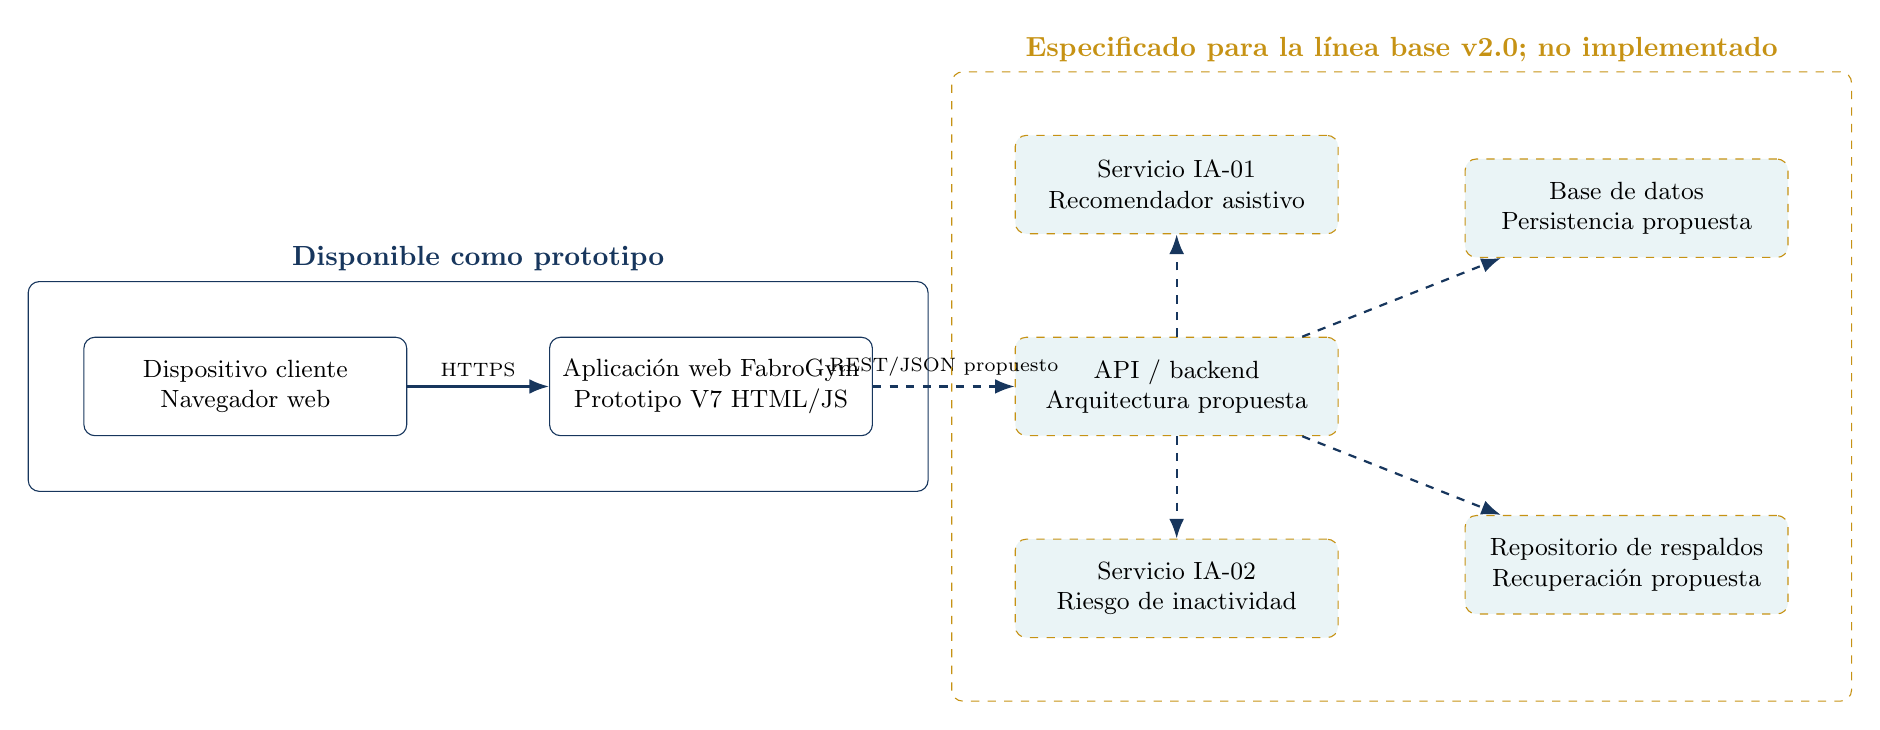
\begin{tikzpicture}[node distance=13mm and 18mm]
\node[nodebox] (browser) {Dispositivo cliente\\Navegador web};
\node[nodebox,right=of browser] (front) {Aplicación web FabroGym\\Prototipo V7 HTML/JS};
\node[future,right=of front] (api) {API / backend\\Arquitectura propuesta};
\node[future,above right=10mm and 16mm of api] (db) {Base de datos\\Persistencia propuesta};
\node[future,below right=10mm and 16mm of api] (bck) {Repositorio de respaldos\\Recuperación propuesta};
\node[future,above=of api] (iar) {Servicio IA-01\\Recomendador asistivo};
\node[future,below=of api] (iaa) {Servicio IA-02\\Riesgo de inactividad};
\draw[flow] (browser)--node[above,font=\scriptsize]{HTTPS}(front);
\draw[flow,dashed] (front)--node[above,font=\scriptsize]{REST/JSON propuesto}(api);
\draw[flow,dashed] (api)--(db); \draw[flow,dashed] (api)--(bck);
\draw[flow,dashed] (api)--(iar); \draw[flow,dashed] (api)--(iaa);
\node[draw=navy,rounded corners,fit=(browser)(front),inner sep=7mm,label={[font=\bfseries,text=navy]above:Disponible como prototipo}] {};
\node[draw=gold,dashed,rounded corners,fit=(api)(db)(bck)(iar)(iaa),inner sep=8mm,label={[font=\bfseries,text=gold]above:Especificado para la línea base v2.0; no implementado}] {};
\end{tikzpicture}\end{document}

